% Options for packages loaded elsewhere
\PassOptionsToPackage{unicode}{hyperref}
\PassOptionsToPackage{hyphens}{url}
\PassOptionsToPackage{dvipsnames,svgnames,x11names}{xcolor}
%
\documentclass[
  letterpaper,
  DIV=11,
  numbers=noendperiod]{scrartcl}

\usepackage{amsmath,amssymb}
\usepackage{iftex}
\ifPDFTeX
  \usepackage[T1]{fontenc}
  \usepackage[utf8]{inputenc}
  \usepackage{textcomp} % provide euro and other symbols
\else % if luatex or xetex
  \usepackage{unicode-math}
  \defaultfontfeatures{Scale=MatchLowercase}
  \defaultfontfeatures[\rmfamily]{Ligatures=TeX,Scale=1}
\fi
\usepackage{lmodern}
\ifPDFTeX\else  
    % xetex/luatex font selection
\fi
% Use upquote if available, for straight quotes in verbatim environments
\IfFileExists{upquote.sty}{\usepackage{upquote}}{}
\IfFileExists{microtype.sty}{% use microtype if available
  \usepackage[]{microtype}
  \UseMicrotypeSet[protrusion]{basicmath} % disable protrusion for tt fonts
}{}
\makeatletter
\@ifundefined{KOMAClassName}{% if non-KOMA class
  \IfFileExists{parskip.sty}{%
    \usepackage{parskip}
  }{% else
    \setlength{\parindent}{0pt}
    \setlength{\parskip}{6pt plus 2pt minus 1pt}}
}{% if KOMA class
  \KOMAoptions{parskip=half}}
\makeatother
\usepackage{xcolor}
\setlength{\emergencystretch}{3em} % prevent overfull lines
\setcounter{secnumdepth}{5}
% Make \paragraph and \subparagraph free-standing
\makeatletter
\ifx\paragraph\undefined\else
  \let\oldparagraph\paragraph
  \renewcommand{\paragraph}{
    \@ifstar
      \xxxParagraphStar
      \xxxParagraphNoStar
  }
  \newcommand{\xxxParagraphStar}[1]{\oldparagraph*{#1}\mbox{}}
  \newcommand{\xxxParagraphNoStar}[1]{\oldparagraph{#1}\mbox{}}
\fi
\ifx\subparagraph\undefined\else
  \let\oldsubparagraph\subparagraph
  \renewcommand{\subparagraph}{
    \@ifstar
      \xxxSubParagraphStar
      \xxxSubParagraphNoStar
  }
  \newcommand{\xxxSubParagraphStar}[1]{\oldsubparagraph*{#1}\mbox{}}
  \newcommand{\xxxSubParagraphNoStar}[1]{\oldsubparagraph{#1}\mbox{}}
\fi
\makeatother

\usepackage{color}
\usepackage{fancyvrb}
\newcommand{\VerbBar}{|}
\newcommand{\VERB}{\Verb[commandchars=\\\{\}]}
\DefineVerbatimEnvironment{Highlighting}{Verbatim}{commandchars=\\\{\}}
% Add ',fontsize=\small' for more characters per line
\usepackage{framed}
\definecolor{shadecolor}{RGB}{241,243,245}
\newenvironment{Shaded}{\begin{snugshade}}{\end{snugshade}}
\newcommand{\AlertTok}[1]{\textcolor[rgb]{0.68,0.00,0.00}{#1}}
\newcommand{\AnnotationTok}[1]{\textcolor[rgb]{0.37,0.37,0.37}{#1}}
\newcommand{\AttributeTok}[1]{\textcolor[rgb]{0.40,0.45,0.13}{#1}}
\newcommand{\BaseNTok}[1]{\textcolor[rgb]{0.68,0.00,0.00}{#1}}
\newcommand{\BuiltInTok}[1]{\textcolor[rgb]{0.00,0.23,0.31}{#1}}
\newcommand{\CharTok}[1]{\textcolor[rgb]{0.13,0.47,0.30}{#1}}
\newcommand{\CommentTok}[1]{\textcolor[rgb]{0.37,0.37,0.37}{#1}}
\newcommand{\CommentVarTok}[1]{\textcolor[rgb]{0.37,0.37,0.37}{\textit{#1}}}
\newcommand{\ConstantTok}[1]{\textcolor[rgb]{0.56,0.35,0.01}{#1}}
\newcommand{\ControlFlowTok}[1]{\textcolor[rgb]{0.00,0.23,0.31}{\textbf{#1}}}
\newcommand{\DataTypeTok}[1]{\textcolor[rgb]{0.68,0.00,0.00}{#1}}
\newcommand{\DecValTok}[1]{\textcolor[rgb]{0.68,0.00,0.00}{#1}}
\newcommand{\DocumentationTok}[1]{\textcolor[rgb]{0.37,0.37,0.37}{\textit{#1}}}
\newcommand{\ErrorTok}[1]{\textcolor[rgb]{0.68,0.00,0.00}{#1}}
\newcommand{\ExtensionTok}[1]{\textcolor[rgb]{0.00,0.23,0.31}{#1}}
\newcommand{\FloatTok}[1]{\textcolor[rgb]{0.68,0.00,0.00}{#1}}
\newcommand{\FunctionTok}[1]{\textcolor[rgb]{0.28,0.35,0.67}{#1}}
\newcommand{\ImportTok}[1]{\textcolor[rgb]{0.00,0.46,0.62}{#1}}
\newcommand{\InformationTok}[1]{\textcolor[rgb]{0.37,0.37,0.37}{#1}}
\newcommand{\KeywordTok}[1]{\textcolor[rgb]{0.00,0.23,0.31}{\textbf{#1}}}
\newcommand{\NormalTok}[1]{\textcolor[rgb]{0.00,0.23,0.31}{#1}}
\newcommand{\OperatorTok}[1]{\textcolor[rgb]{0.37,0.37,0.37}{#1}}
\newcommand{\OtherTok}[1]{\textcolor[rgb]{0.00,0.23,0.31}{#1}}
\newcommand{\PreprocessorTok}[1]{\textcolor[rgb]{0.68,0.00,0.00}{#1}}
\newcommand{\RegionMarkerTok}[1]{\textcolor[rgb]{0.00,0.23,0.31}{#1}}
\newcommand{\SpecialCharTok}[1]{\textcolor[rgb]{0.37,0.37,0.37}{#1}}
\newcommand{\SpecialStringTok}[1]{\textcolor[rgb]{0.13,0.47,0.30}{#1}}
\newcommand{\StringTok}[1]{\textcolor[rgb]{0.13,0.47,0.30}{#1}}
\newcommand{\VariableTok}[1]{\textcolor[rgb]{0.07,0.07,0.07}{#1}}
\newcommand{\VerbatimStringTok}[1]{\textcolor[rgb]{0.13,0.47,0.30}{#1}}
\newcommand{\WarningTok}[1]{\textcolor[rgb]{0.37,0.37,0.37}{\textit{#1}}}

\providecommand{\tightlist}{%
  \setlength{\itemsep}{0pt}\setlength{\parskip}{0pt}}\usepackage{longtable,booktabs,array}
\usepackage{calc} % for calculating minipage widths
% Correct order of tables after \paragraph or \subparagraph
\usepackage{etoolbox}
\makeatletter
\patchcmd\longtable{\par}{\if@noskipsec\mbox{}\fi\par}{}{}
\makeatother
% Allow footnotes in longtable head/foot
\IfFileExists{footnotehyper.sty}{\usepackage{footnotehyper}}{\usepackage{footnote}}
\makesavenoteenv{longtable}
\usepackage{graphicx}
\makeatletter
\def\maxwidth{\ifdim\Gin@nat@width>\linewidth\linewidth\else\Gin@nat@width\fi}
\def\maxheight{\ifdim\Gin@nat@height>\textheight\textheight\else\Gin@nat@height\fi}
\makeatother
% Scale images if necessary, so that they will not overflow the page
% margins by default, and it is still possible to overwrite the defaults
% using explicit options in \includegraphics[width, height, ...]{}
\setkeys{Gin}{width=\maxwidth,height=\maxheight,keepaspectratio}
% Set default figure placement to htbp
\makeatletter
\def\fps@figure{htbp}
\makeatother

\usepackage{booktabs}
\usepackage{caption}
\usepackage{longtable}
\usepackage{colortbl}
\usepackage{array}
\usepackage{anyfontsize}
\usepackage{multirow}
\KOMAoption{captions}{tableheading}
\makeatletter
\@ifpackageloaded{caption}{}{\usepackage{caption}}
\AtBeginDocument{%
\ifdefined\contentsname
  \renewcommand*\contentsname{Table of contents}
\else
  \newcommand\contentsname{Table of contents}
\fi
\ifdefined\listfigurename
  \renewcommand*\listfigurename{List of Figures}
\else
  \newcommand\listfigurename{List of Figures}
\fi
\ifdefined\listtablename
  \renewcommand*\listtablename{List of Tables}
\else
  \newcommand\listtablename{List of Tables}
\fi
\ifdefined\figurename
  \renewcommand*\figurename{Figure}
\else
  \newcommand\figurename{Figure}
\fi
\ifdefined\tablename
  \renewcommand*\tablename{Table}
\else
  \newcommand\tablename{Table}
\fi
}
\@ifpackageloaded{float}{}{\usepackage{float}}
\floatstyle{ruled}
\@ifundefined{c@chapter}{\newfloat{codelisting}{h}{lop}}{\newfloat{codelisting}{h}{lop}[chapter]}
\floatname{codelisting}{Listing}
\newcommand*\listoflistings{\listof{codelisting}{List of Listings}}
\makeatother
\makeatletter
\makeatother
\makeatletter
\@ifpackageloaded{caption}{}{\usepackage{caption}}
\@ifpackageloaded{subcaption}{}{\usepackage{subcaption}}
\makeatother

\ifLuaTeX
  \usepackage{selnolig}  % disable illegal ligatures
\fi
\usepackage{bookmark}

\IfFileExists{xurl.sty}{\usepackage{xurl}}{} % add URL line breaks if available
\urlstyle{same} % disable monospaced font for URLs
\hypersetup{
  pdftitle={Mini-Project \#04: Monte Carlo-Informed Selection of CUNY Retirement Plans},
  colorlinks=true,
  linkcolor={blue},
  filecolor={Maroon},
  citecolor={Blue},
  urlcolor={Blue},
  pdfcreator={LaTeX via pandoc}}


\title{Mini-Project \#04: Monte Carlo-Informed Selection of CUNY
Retirement Plans}
\author{}
\date{}

\begin{document}
\maketitle

\renewcommand*\contentsname{Outline}
{
\hypersetup{linkcolor=}
\setcounter{tocdepth}{2}
\tableofcontents
}

\subsection{Introduction}\label{introduction}

Choosing a retirement plan is a critical decision for new CUNY faculty,
who must select between the \textbf{Teachers Retirement System (TRS)}
and the \textbf{Optional Retirement Plan (ORP)} within 30 days. The TRS
is a defined-benefit plan that provides predictable lifetime income
based on salary and years of service, with contributions and inflation
adjustments structured to ensure steady growth. In contrast, the ORP is
a defined-contribution plan, where savings depend on market performance,
offering more flexibility but shifting the investment risk to employees.

This research uses financial modeling in R to evaluate the long-term
outcomes of these plans. By simulating market returns, inflation
adjustments, and compound interest, we aim to estimate which plan is
likely to provide greater financial benefits. This project highlights
the power of data-driven analysis in making informed financial
decisions.

\begin{Shaded}
\begin{Highlighting}[]
\FunctionTok{library}\NormalTok{(lubridate)}
\FunctionTok{library}\NormalTok{(httr2)}
\FunctionTok{library}\NormalTok{(dplyr)}
\FunctionTok{library}\NormalTok{(ggplot2)}
\FunctionTok{library}\NormalTok{(tidyr)}
\FunctionTok{library}\NormalTok{(fuzzyjoin)}
\FunctionTok{library}\NormalTok{(purrr)}
\FunctionTok{library}\NormalTok{(tibble) }\CommentTok{\#rownames\_to\_column bug}
\FunctionTok{library}\NormalTok{(DT)}
\FunctionTok{library}\NormalTok{(jsonlite)}
\FunctionTok{library}\NormalTok{(stringr)}
\FunctionTok{library}\NormalTok{(gt)}
\end{Highlighting}
\end{Shaded}

\subsection{Data Sources - AlphaVantage \&
FRED}\label{data-sources---alphavantage-fred}

For this project, we will use data from two economic and financial data
sources:

\begin{itemize}
\item
  \href{https://www.alphavantage.co/}{AlphaVantage}: a commercial stock
  market data provider
\item
  \href{https://fred.stlouisfed.org/}{FRED}: the Federal Reserve
  Economic Data repository maintained by the Federal Reserve Bank of
  St.~Louis
\end{itemize}

From AlphaVantage, we are extracting \textbf{adjusted close prices} for
selected financial instruments (e.g., U.S. equities -- SPY,
international equities, and bonds). This data helps analyze trends,
calculate returns, and measure compounding growth.

\begin{Shaded}
\begin{Highlighting}[]
\NormalTok{alpha\_vantage\_key }\OtherTok{\textless{}{-}} \FunctionTok{readLines}\NormalTok{(}\StringTok{"AlphaKey.txt"}\NormalTok{)}
\CommentTok{\# Define a function to fetch data from Alpha Vantage}
\NormalTok{get\_alpha\_data }\OtherTok{\textless{}{-}} \ControlFlowTok{function}\NormalTok{(symbol, }\AttributeTok{interval =} \StringTok{"TIME\_SERIES\_DAILY"}\NormalTok{, api\_key) \{}
\NormalTok{  url }\OtherTok{\textless{}{-}} \FunctionTok{paste0}\NormalTok{(}\StringTok{"https://www.alphavantage.co/query?function="}\NormalTok{, interval,}
                \StringTok{"\&symbol="}\NormalTok{, symbol, }\StringTok{"\&apikey="}\NormalTok{, api\_key, }\StringTok{"\&outputsize=full\&datatype=json"}\NormalTok{)}
  
  \CommentTok{\# Send request and check response}
\NormalTok{  response }\OtherTok{\textless{}{-}} \FunctionTok{request}\NormalTok{(url) }\SpecialCharTok{\%\textgreater{}\%} \FunctionTok{req\_perform}\NormalTok{()}
  \ControlFlowTok{if}\NormalTok{ (response }\SpecialCharTok{\%\textgreater{}\%} \FunctionTok{resp\_status}\NormalTok{() }\SpecialCharTok{!=} \DecValTok{200}\NormalTok{) \{}
    \FunctionTok{stop}\NormalTok{(}\StringTok{"Failed to retrieve Alpha Vantage data. HTTP Status: "}\NormalTok{, response }\SpecialCharTok{\%\textgreater{}\%} \FunctionTok{resp\_status}\NormalTok{())}
\NormalTok{  \}}
  
\NormalTok{  data }\OtherTok{\textless{}{-}} \FunctionTok{fromJSON}\NormalTok{(response }\SpecialCharTok{\%\textgreater{}\%} \FunctionTok{resp\_body\_string}\NormalTok{())}
\NormalTok{  timeseries }\OtherTok{\textless{}{-}}\NormalTok{ data[[}\StringTok{"Time Series (Daily)"}\NormalTok{]]}
  \ControlFlowTok{if}\NormalTok{ (}\FunctionTok{is.null}\NormalTok{(timeseries)) }\FunctionTok{stop}\NormalTok{(}\StringTok{"Failed to retrieve Alpha Vantage data for symbol: "}\NormalTok{, symbol)}
  
\NormalTok{  df }\OtherTok{\textless{}{-}} \FunctionTok{as.data.frame}\NormalTok{(}\FunctionTok{do.call}\NormalTok{(rbind, timeseries))}
\NormalTok{  df}\SpecialCharTok{$}\NormalTok{date }\OtherTok{\textless{}{-}} \FunctionTok{rownames}\NormalTok{(df)}
  \FunctionTok{rownames}\NormalTok{(df) }\OtherTok{\textless{}{-}} \ConstantTok{NULL}
  
  \CommentTok{\# Data cleaning and processing}
\NormalTok{  df }\OtherTok{\textless{}{-}}\NormalTok{ df }\SpecialCharTok{\%\textgreater{}\%}
    \FunctionTok{rename}\NormalTok{(}\AttributeTok{close =} \StringTok{\textasciigrave{}}\AttributeTok{4. close}\StringTok{\textasciigrave{}}\NormalTok{) }\SpecialCharTok{\%\textgreater{}\%}
    \FunctionTok{mutate}\NormalTok{(}
      \AttributeTok{date =} \FunctionTok{as.Date}\NormalTok{(date),}
      \AttributeTok{close =} \FunctionTok{as.numeric}\NormalTok{(close)}
\NormalTok{    ) }\SpecialCharTok{\%\textgreater{}\%}
    \FunctionTok{arrange}\NormalTok{(date)}
  
\NormalTok{  df }\OtherTok{\textless{}{-}}\NormalTok{ df }\SpecialCharTok{\%\textgreater{}\%}
    \FunctionTok{mutate}\NormalTok{(}\AttributeTok{month =} \FunctionTok{format}\NormalTok{(date, }\StringTok{"\%Y{-}\%m"}\NormalTok{)) }\SpecialCharTok{\%\textgreater{}\%}
    \FunctionTok{group\_by}\NormalTok{(month) }\SpecialCharTok{\%\textgreater{}\%}
    \FunctionTok{summarize}\NormalTok{(}
      \AttributeTok{monthly\_return =} \FunctionTok{last}\NormalTok{(close) }\SpecialCharTok{/} \FunctionTok{first}\NormalTok{(close) }\SpecialCharTok{{-}} \DecValTok{1}\NormalTok{,}
      \AttributeTok{.groups =} \StringTok{\textquotesingle{}drop\textquotesingle{}}
\NormalTok{    ) }\SpecialCharTok{\%\textgreater{}\%}
    \FunctionTok{mutate}\NormalTok{(}\AttributeTok{date =} \FunctionTok{as.Date}\NormalTok{(}\FunctionTok{paste0}\NormalTok{(month, }\StringTok{"{-}01"}\NormalTok{))) }\SpecialCharTok{\%\textgreater{}\%}
    \FunctionTok{select}\NormalTok{(date, monthly\_return)}
  
  \FunctionTok{return}\NormalTok{(df)}
\NormalTok{\}}
\end{Highlighting}
\end{Shaded}

From FRED, we are extracting economic indicators such as inflation
(CPI), wage growth, and short-term treasury yields. These metrics are
vital for modeling economic trends and understanding how they relate to
investments.

\begin{Shaded}
\begin{Highlighting}[]
\NormalTok{fred\_key }\OtherTok{\textless{}{-}} \FunctionTok{readLines}\NormalTok{(}\StringTok{"FredKey.txt"}\NormalTok{)}
\CommentTok{\# Define a function to fetch data from FRED}
\NormalTok{get\_fred\_data }\OtherTok{\textless{}{-}} \ControlFlowTok{function}\NormalTok{(series\_id, api\_key) \{}
\NormalTok{  url }\OtherTok{\textless{}{-}} \FunctionTok{paste0}\NormalTok{(}\StringTok{"https://api.stlouisfed.org/fred/series/observations?series\_id="}\NormalTok{, }
\NormalTok{                series\_id, }\StringTok{"\&api\_key="}\NormalTok{, api\_key, }\StringTok{"\&file\_type=json"}\NormalTok{)}
  
  \CommentTok{\# Send request and check response}
\NormalTok{  response }\OtherTok{\textless{}{-}} \FunctionTok{request}\NormalTok{(url) }\SpecialCharTok{\%\textgreater{}\%} \FunctionTok{req\_perform}\NormalTok{()}
  \ControlFlowTok{if}\NormalTok{ (response }\SpecialCharTok{\%\textgreater{}\%} \FunctionTok{resp\_status}\NormalTok{() }\SpecialCharTok{!=} \DecValTok{200}\NormalTok{) \{}
    \FunctionTok{stop}\NormalTok{(}\StringTok{"Failed to retrieve FRED data. HTTP Status: "}\NormalTok{, response }\SpecialCharTok{\%\textgreater{}\%} \FunctionTok{resp\_status}\NormalTok{())}
\NormalTok{  \}}
  
  \CommentTok{\# Parse JSON response}
\NormalTok{  data }\OtherTok{\textless{}{-}} \FunctionTok{fromJSON}\NormalTok{(response }\SpecialCharTok{\%\textgreater{}\%} \FunctionTok{resp\_body\_string}\NormalTok{())}
  \ControlFlowTok{if}\NormalTok{ (}\FunctionTok{is.null}\NormalTok{(data}\SpecialCharTok{$}\NormalTok{observations)) }\FunctionTok{stop}\NormalTok{(}\StringTok{"No observations found for series: "}\NormalTok{, series\_id)}
  
  \CommentTok{\# Convert to data frame}
\NormalTok{  df }\OtherTok{\textless{}{-}} \FunctionTok{as.data.frame}\NormalTok{(data}\SpecialCharTok{$}\NormalTok{observations) }\SpecialCharTok{\%\textgreater{}\%}
    \FunctionTok{mutate}\NormalTok{(}
      \AttributeTok{date =} \FunctionTok{as.Date}\NormalTok{(date),}
      \AttributeTok{value =} \FunctionTok{suppressWarnings}\NormalTok{(}\FunctionTok{as.numeric}\NormalTok{(value))}
\NormalTok{    ) }\SpecialCharTok{\%\textgreater{}\%}
    \FunctionTok{filter}\NormalTok{(}\SpecialCharTok{!}\FunctionTok{is.na}\NormalTok{(value)) }\SpecialCharTok{\%\textgreater{}\%}
    \FunctionTok{select}\NormalTok{(date, value)}
  
  \FunctionTok{return}\NormalTok{(df)}
\NormalTok{\}}
\end{Highlighting}
\end{Shaded}

\subsection{Data Acquisition}\label{data-acquisition}

For our Monte Carlo analysis, we need a comprehensive dataset covering
historical trends in wage growth, inflation, and market returns across
different asset classes. Specifically, we will extract:

\begin{enumerate}
\def\labelenumi{\arabic{enumi}.}
\item
  \textbf{Wage Growth}: Historical wage growth rates from FRED, using
  the series \texttt{CES0500000003} (Average Hourly Earnings Growth).
\item
  \textbf{Inflation}: Historical inflation data from FRED, using the
  series \texttt{CPIAUCSL} (Consumer Price Index for All Urban
  Consumers).
\item
  \textbf{U.S. Stock Market Returns}: Adjusted close prices for the SPY
  ETF (a proxy for U.S. equities) from AlphaVantage.
\item
  \textbf{International Stock Market Returns}: Adjusted close prices for
  the ACWI ETF (a proxy for international equities) from AlphaVantage.
\item
  \textbf{Bond Market Returns}: Historical yields for 10-Year Treasury
  Bonds from FRED, using the series \texttt{GS10}.
\item
  \textbf{Short-Term Debt Returns}: Historical yields for 2-Year
  Treasury Bonds from FRED, using the series \texttt{DGS2}.
\end{enumerate}

\begin{Shaded}
\begin{Highlighting}[]
\NormalTok{wage\_growth\_data }\OtherTok{\textless{}{-}} \FunctionTok{get\_fred\_data}\NormalTok{(}\StringTok{"CES0500000003"}\NormalTok{, fred\_key) }\SpecialCharTok{\%\textgreater{}\%}
  \FunctionTok{mutate}\NormalTok{(}\AttributeTok{month =} \FunctionTok{format}\NormalTok{(date, }\StringTok{"\%Y{-}\%m"}\NormalTok{)) }\SpecialCharTok{\%\textgreater{}\%}
  \FunctionTok{group\_by}\NormalTok{(month) }\SpecialCharTok{\%\textgreater{}\%}
  \FunctionTok{summarize}\NormalTok{(}\AttributeTok{wage\_growth\_rate =} \FunctionTok{last}\NormalTok{(value), }\AttributeTok{.groups =} \StringTok{\textquotesingle{}drop\textquotesingle{}}\NormalTok{) }\SpecialCharTok{\%\textgreater{}\%}
  \FunctionTok{mutate}\NormalTok{(}\AttributeTok{date =} \FunctionTok{as.Date}\NormalTok{(}\FunctionTok{paste0}\NormalTok{(month, }\StringTok{"{-}01"}\NormalTok{))) }\SpecialCharTok{\%\textgreater{}\%}
  \FunctionTok{select}\NormalTok{(date, wage\_growth\_rate)}

\NormalTok{inflation\_data }\OtherTok{\textless{}{-}} \FunctionTok{get\_fred\_data}\NormalTok{(}\StringTok{"CPIAUCSL"}\NormalTok{, fred\_key) }\SpecialCharTok{\%\textgreater{}\%}
  \FunctionTok{mutate}\NormalTok{(}\AttributeTok{month =} \FunctionTok{format}\NormalTok{(date, }\StringTok{"\%Y{-}\%m"}\NormalTok{)) }\SpecialCharTok{\%\textgreater{}\%}
  \FunctionTok{group\_by}\NormalTok{(month) }\SpecialCharTok{\%\textgreater{}\%}
  \FunctionTok{summarize}\NormalTok{(}\AttributeTok{inflation\_rate =} \FunctionTok{last}\NormalTok{(value), }\AttributeTok{.groups =} \StringTok{\textquotesingle{}drop\textquotesingle{}}\NormalTok{) }\SpecialCharTok{\%\textgreater{}\%}
  \FunctionTok{mutate}\NormalTok{(}\AttributeTok{date =} \FunctionTok{as.Date}\NormalTok{(}\FunctionTok{paste0}\NormalTok{(month, }\StringTok{"{-}01"}\NormalTok{))) }\SpecialCharTok{\%\textgreater{}\%}
  \FunctionTok{select}\NormalTok{(date, inflation\_rate)}

\NormalTok{us\_equity\_data }\OtherTok{\textless{}{-}} \FunctionTok{get\_alpha\_data}\NormalTok{(}\StringTok{"SPY"}\NormalTok{, }\StringTok{"TIME\_SERIES\_DAILY"}\NormalTok{, alpha\_vantage\_key) }\SpecialCharTok{\%\textgreater{}\%}
  \FunctionTok{rename}\NormalTok{(}\AttributeTok{us\_equity\_return =}\NormalTok{ monthly\_return)}

\NormalTok{intl\_equity\_data }\OtherTok{\textless{}{-}} \FunctionTok{get\_alpha\_data}\NormalTok{(}\StringTok{"ACWI"}\NormalTok{, }\StringTok{"TIME\_SERIES\_DAILY"}\NormalTok{, alpha\_vantage\_key) }\SpecialCharTok{\%\textgreater{}\%}
  \FunctionTok{rename}\NormalTok{(}\AttributeTok{intl\_equity\_return =}\NormalTok{ monthly\_return)}

\NormalTok{bond\_data }\OtherTok{\textless{}{-}} \FunctionTok{get\_fred\_data}\NormalTok{(}\StringTok{"GS10"}\NormalTok{, fred\_key) }\SpecialCharTok{\%\textgreater{}\%}
  \FunctionTok{mutate}\NormalTok{(}\AttributeTok{month =} \FunctionTok{format}\NormalTok{(date, }\StringTok{"\%Y{-}\%m"}\NormalTok{)) }\SpecialCharTok{\%\textgreater{}\%}
  \FunctionTok{group\_by}\NormalTok{(month) }\SpecialCharTok{\%\textgreater{}\%}
  \FunctionTok{summarize}\NormalTok{(}\AttributeTok{bond\_return =} \FunctionTok{last}\NormalTok{(value), }\AttributeTok{.groups =} \StringTok{\textquotesingle{}drop\textquotesingle{}}\NormalTok{) }\SpecialCharTok{\%\textgreater{}\%}
  \FunctionTok{mutate}\NormalTok{(}\AttributeTok{date =} \FunctionTok{as.Date}\NormalTok{(}\FunctionTok{paste0}\NormalTok{(month, }\StringTok{"{-}01"}\NormalTok{))) }\SpecialCharTok{\%\textgreater{}\%}
  \FunctionTok{select}\NormalTok{(date, bond\_return)}

\NormalTok{short\_term\_debt\_data }\OtherTok{\textless{}{-}} \FunctionTok{get\_fred\_data}\NormalTok{(}\StringTok{"DGS2"}\NormalTok{, fred\_key) }\SpecialCharTok{\%\textgreater{}\%}
  \FunctionTok{mutate}\NormalTok{(}\AttributeTok{month =} \FunctionTok{format}\NormalTok{(date, }\StringTok{"\%Y{-}\%m"}\NormalTok{)) }\SpecialCharTok{\%\textgreater{}\%}
  \FunctionTok{group\_by}\NormalTok{(month) }\SpecialCharTok{\%\textgreater{}\%}
  \FunctionTok{summarize}\NormalTok{(}\AttributeTok{short\_term\_rate =} \FunctionTok{last}\NormalTok{(value), }\AttributeTok{.groups =} \StringTok{\textquotesingle{}drop\textquotesingle{}}\NormalTok{) }\SpecialCharTok{\%\textgreater{}\%}
  \FunctionTok{mutate}\NormalTok{(}\AttributeTok{date =} \FunctionTok{as.Date}\NormalTok{(}\FunctionTok{paste0}\NormalTok{(month, }\StringTok{"{-}01"}\NormalTok{))) }\SpecialCharTok{\%\textgreater{}\%}
  \FunctionTok{select}\NormalTok{(date, short\_term\_rate)}

\NormalTok{all\_data }\OtherTok{\textless{}{-}} \FunctionTok{list}\NormalTok{(}
\NormalTok{  wage\_growth\_data,}
\NormalTok{  inflation\_data,}
\NormalTok{  us\_equity\_data,}
\NormalTok{  intl\_equity\_data,}
\NormalTok{  bond\_data,}
\NormalTok{  short\_term\_debt\_data}
\NormalTok{) }\SpecialCharTok{\%\textgreater{}\%}
  \FunctionTok{reduce}\NormalTok{(full\_join, }\AttributeTok{by =} \StringTok{"date"}\NormalTok{) }\SpecialCharTok{\%\textgreater{}\%}
  \FunctionTok{arrange}\NormalTok{(date) }\SpecialCharTok{\%\textgreater{}\%}
  \FunctionTok{drop\_na}\NormalTok{()  }
\end{Highlighting}
\end{Shaded}

\subsection{Detailed Analysis of
Correlations}\label{detailed-analysis-of-correlations}

\paragraph{\texorpdfstring{\textbf{1. Wage Growth Rate and Inflation
Rate (Correlation:
0.99)}}{1. Wage Growth Rate and Inflation Rate (Correlation: 0.99)}}\label{wage-growth-rate-and-inflation-rate-correlation-0.99}

Wage growth and inflation are almost perfectly correlated, with a
coefficient of \textbf{0.99}. This strong relationship suggests that as
inflation rises, wages tend to adjust upward to maintain purchasing
power. However, the lag effect between inflation increases and wage
adjustments may still impact real income, as wage growth may not
immediately match inflation in real-time. This high correlation also
reflects how labor markets react to price-level changes in the economy.

\paragraph{\texorpdfstring{\textbf{2. U.S. Stock Market and
International Stock Market Returns (Correlation:
0.97)}}{2. U.S. Stock Market and International Stock Market Returns (Correlation: 0.97)}}\label{u.s.-stock-market-and-international-stock-market-returns-correlation-0.97}

The correlation between U.S. equity returns (SPY) and international
equity returns (ACWI) is \textbf{0.97}, indicating that these markets
tend to move together. Global economic factors, such as monetary
policies, geopolitical events, or trade relationships, likely drive this
interdependence.

\paragraph{\texorpdfstring{\textbf{3. Bond Returns vs.~Short-Term Debt
Returns (Correlation:
0.71)}}{3. Bond Returns vs.~Short-Term Debt Returns (Correlation: 0.71)}}\label{bond-returns-vs.-short-term-debt-returns-correlation-0.71}

A moderately strong correlation of \textbf{0.71} between bond returns
(10-year Treasury yields) and short-term debt returns (2-year Treasury
yields) reflects the influence of the yield curve. Both long-term and
short-term rates are sensitive to interest rate changes, but they
respond differently to economic conditions.

\paragraph{\texorpdfstring{\textbf{4. Inflation Rate vs.~Short-Term Debt
Returns (Correlation:
0.74)}}{4. Inflation Rate vs.~Short-Term Debt Returns (Correlation: 0.74)}}\label{inflation-rate-vs.-short-term-debt-returns-correlation-0.74}

The correlation between inflation and short-term debt returns is
\textbf{0.74}, reflecting that short-term interest rates rise in
response to inflationary pressures. Central banks typically increase
interest rates to control inflation, which directly impacts short-term
debt yields.

\paragraph{\texorpdfstring{\textbf{5. Stock Market vs.~Other Economic
Indicators}}{5. Stock Market vs.~Other Economic Indicators}}\label{stock-market-vs.-other-economic-indicators}

\begin{itemize}
\item
  The correlation between wage growth and U.S. equity returns is
  \textbf{0.07}, and with international equity returns, it is
  \textbf{0.05}.
\item
  The correlation between inflation and U.S. equity returns is
  \textbf{0.05}, and with international equity returns, it is
  \textbf{0.03}.
\item
  Short-term rates are negatively correlated with U.S. equity returns
  (\textbf{−0.04}) and international equity returns (\textbf{−0.03}).
\item
  Bond returns are weakly negatively correlated with U.S. equity returns
  (\textbf{−0.09}) and international equity returns (\textbf{−0.08}).
\end{itemize}

\begin{Shaded}
\begin{Highlighting}[]
\NormalTok{correlation\_matrix }\OtherTok{\textless{}{-}}\NormalTok{ all\_data }\SpecialCharTok{\%\textgreater{}\%}
  \FunctionTok{select}\NormalTok{(}\SpecialCharTok{{-}}\NormalTok{date) }\SpecialCharTok{\%\textgreater{}\%}
  \FunctionTok{cor}\NormalTok{(}\AttributeTok{use =} \StringTok{"complete.obs"}\NormalTok{)}
\NormalTok{correlation\_data }\OtherTok{\textless{}{-}}\NormalTok{ correlation\_matrix }\SpecialCharTok{\%\textgreater{}\%}
  \FunctionTok{as\_tibble}\NormalTok{(}\AttributeTok{rownames =} \StringTok{"Variable1"}\NormalTok{) }\SpecialCharTok{\%\textgreater{}\%}
  \FunctionTok{pivot\_longer}\NormalTok{(}\AttributeTok{cols =} \SpecialCharTok{{-}}\NormalTok{Variable1, }\AttributeTok{names\_to =} \StringTok{"Variable2"}\NormalTok{, }\AttributeTok{values\_to =} \StringTok{"Correlation"}\NormalTok{)}

\FunctionTok{ggplot}\NormalTok{(correlation\_data, }\FunctionTok{aes}\NormalTok{(}\AttributeTok{x =}\NormalTok{ Variable1, }\AttributeTok{y =}\NormalTok{ Variable2, }\AttributeTok{fill =}\NormalTok{ Correlation)) }\SpecialCharTok{+}
  \FunctionTok{geom\_tile}\NormalTok{(}\AttributeTok{color =} \StringTok{"white"}\NormalTok{) }\SpecialCharTok{+}
  \FunctionTok{scale\_fill\_gradient2}\NormalTok{(}\AttributeTok{low =} \StringTok{"lightblue"}\NormalTok{, }\AttributeTok{mid =} \StringTok{"white"}\NormalTok{, }\AttributeTok{high =} \StringTok{"darkblue"}\NormalTok{, }\AttributeTok{midpoint =} \DecValTok{0}\NormalTok{) }\SpecialCharTok{+}
  \FunctionTok{theme\_minimal}\NormalTok{() }\SpecialCharTok{+}
  \FunctionTok{labs}\NormalTok{(}
    \AttributeTok{title =} \StringTok{"Correlation Heatmap"}\NormalTok{,}
    \AttributeTok{x =} \StringTok{"Indicator 1"}\NormalTok{,}
    \AttributeTok{y =} \StringTok{"Indicator 2"}\NormalTok{,}
    \AttributeTok{fill =} \StringTok{"Correlation"}
\NormalTok{  ) }\SpecialCharTok{+}
  \FunctionTok{theme}\NormalTok{(}
    \AttributeTok{axis.text.x =} \FunctionTok{element\_text}\NormalTok{(}\AttributeTok{angle =} \DecValTok{45}\NormalTok{, }\AttributeTok{hjust =} \DecValTok{1}\NormalTok{),}
    \AttributeTok{panel.grid =} \FunctionTok{element\_blank}\NormalTok{()}
\NormalTok{  )}
\end{Highlighting}
\end{Shaded}

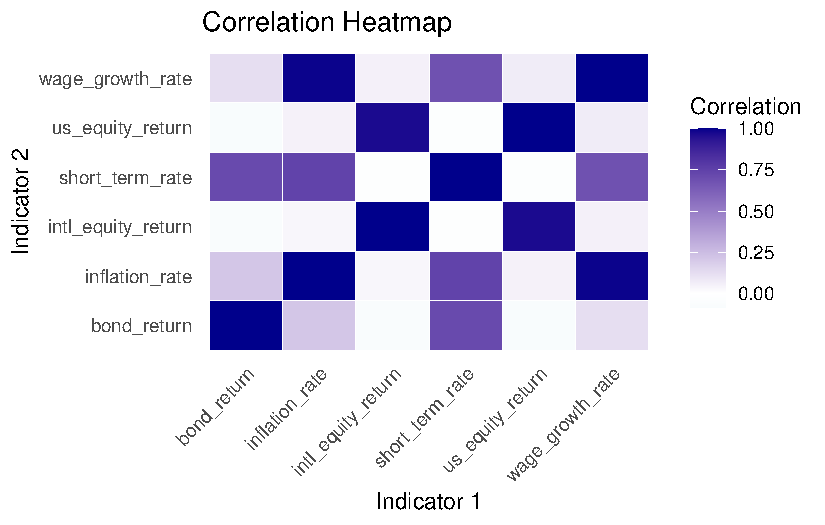
\includegraphics{mp04_files/figure-pdf/unnamed-chunk-5-1.pdf}

\subsection{Summary Statistics
Explanation}\label{summary-statistics-explanation}

\begin{enumerate}
\def\labelenumi{\arabic{enumi}.}
\item
  \textbf{Wage Growth}: Average hourly wage is \$26.69, with moderate
  variability (variance: \$15.78, Standard Deviation (SD): \$3.97). This
  reflects stable long-term growth.
\item
  \textbf{Inflation}: Average CPI is \$249.21, with high variability
  (variance: \$833.04, SD: \$28.86), indicating significant fluctuations
  and economic uncertainty.
\item
  \textbf{U.S. Equity Returns}: Slightly positive average monthly return
  (\$0.01) with low volatility (SD: \$0.05), reflecting consistent
  performance.
\item
  \textbf{International Equity Returns}: Neutral monthly returns
  (\$0.00) and low volatility (SD: \$0.05), similar to U.S. equities,
  indicating stable international markets.
\item
  \textbf{Bond Returns}: Steady average yield of \$2.58, with low
  variability (variance: \$0.85, SD: \$0.92), highlighting bonds as a
  stable long-term investment.
\item
  \textbf{Short-Term Debt Returns}: Average yield of \$1.44, but higher
  variability (variance: \$1.99, SD: \$1.41), showing greater
  sensitivity to interest rate changes.
\end{enumerate}

Inflation demonstrates the highest variability, underscoring its
economic impact. Equities have low volatility with consistent returns,
while short-term debt shows greater instability compared to bonds,
reflecting sensitivity to policy changes.

\begin{Shaded}
\begin{Highlighting}[]
\NormalTok{summary\_stats }\OtherTok{\textless{}{-}}\NormalTok{ all\_data }\SpecialCharTok{\%\textgreater{}\%}
  \FunctionTok{select}\NormalTok{(}\SpecialCharTok{{-}}\NormalTok{date) }\SpecialCharTok{\%\textgreater{}\%}
  \FunctionTok{summarize\_all}\NormalTok{(}\FunctionTok{list}\NormalTok{(}\AttributeTok{mean =}\NormalTok{ mean, }\AttributeTok{var =}\NormalTok{ var, }\AttributeTok{sd =}\NormalTok{ sd), }\AttributeTok{na.rm =} \ConstantTok{TRUE}\NormalTok{) }\SpecialCharTok{\%\textgreater{}\%}
  \FunctionTok{pivot\_longer}\NormalTok{(}\AttributeTok{cols =} \FunctionTok{everything}\NormalTok{(), }\AttributeTok{names\_to =} \StringTok{"Variable\_Stat"}\NormalTok{, }\AttributeTok{values\_to =} \StringTok{"Value"}\NormalTok{) }\SpecialCharTok{\%\textgreater{}\%}
  \FunctionTok{mutate}\NormalTok{(}
    \AttributeTok{Variable =} \FunctionTok{str\_extract}\NormalTok{(Variable\_Stat, }\StringTok{"\^{}[\^{}\_]+"}\NormalTok{),}
    \AttributeTok{Stat =} \FunctionTok{str\_extract}\NormalTok{(Variable\_Stat, }\StringTok{"[\^{}\_]+$"}\NormalTok{)}
\NormalTok{  ) }\SpecialCharTok{\%\textgreater{}\%}
  \FunctionTok{select}\NormalTok{(}\SpecialCharTok{{-}}\NormalTok{Variable\_Stat) }\SpecialCharTok{\%\textgreater{}\%}
  \FunctionTok{pivot\_wider}\NormalTok{(}\AttributeTok{names\_from =} \StringTok{"Stat"}\NormalTok{, }\AttributeTok{values\_from =} \StringTok{"Value"}\NormalTok{)}

\NormalTok{summary\_stats\_table }\OtherTok{\textless{}{-}}\NormalTok{ summary\_stats }\SpecialCharTok{\%\textgreater{}\%}
  \FunctionTok{gt}\NormalTok{() }\SpecialCharTok{\%\textgreater{}\%}
  \FunctionTok{tab\_header}\NormalTok{(}
    \AttributeTok{title =} \StringTok{"Summary Statistics"}\NormalTok{,}
    \AttributeTok{subtitle =} \StringTok{"Mean, Variance, and Standard Deviation of Variables"}
\NormalTok{  ) }\SpecialCharTok{\%\textgreater{}\%}
  \FunctionTok{fmt\_number}\NormalTok{(}
    \AttributeTok{columns =} \FunctionTok{c}\NormalTok{(mean, var, sd),}
    \AttributeTok{decimals =} \DecValTok{2}
\NormalTok{  ) }\SpecialCharTok{\%\textgreater{}\%}
  \FunctionTok{cols\_label}\NormalTok{(}
    \AttributeTok{Variable =} \StringTok{"Variable"}\NormalTok{,}
    \AttributeTok{mean =} \StringTok{"Mean"}\NormalTok{,}
    \AttributeTok{var =} \StringTok{"Variance"}\NormalTok{,}
    \AttributeTok{sd =} \StringTok{"Standard Deviation"}
\NormalTok{  ) }\SpecialCharTok{\%\textgreater{}\%}
  \FunctionTok{tab\_options}\NormalTok{(}
    \AttributeTok{table.width =} \FunctionTok{px}\NormalTok{(}\DecValTok{700}\NormalTok{),}
    \AttributeTok{column\_labels.font.weight =} \StringTok{"bold"}
\NormalTok{  )}
\NormalTok{summary\_stats\_table}
\end{Highlighting}
\end{Shaded}

\begin{table}
\caption*{
{\large Summary Statistics} \\ 
{\small Mean, Variance, and Standard Deviation of Variables}
} 
\fontsize{12.0pt}{14.4pt}\selectfont
\begin{tabular*}{525pt}{@{\extracolsep{\fill}}lrrr}
\toprule
Variable & Mean & Variance & Standard Deviation \\ 
\midrule\addlinespace[2.5pt]
wage & 26.69 & 15.78 & 3.97 \\ 
inflation & 249.21 & 833.04 & 28.86 \\ 
us & 0.01 & 0.00 & 0.05 \\ 
intl & 0.00 & 0.00 & 0.05 \\ 
bond & 2.58 & 0.85 & 0.92 \\ 
short & 1.44 & 1.99 & 1.41 \\ 
\bottomrule
\end{tabular*}
\end{table}

\subsection{Long-Term Monthly Averages
Analysis}\label{long-term-monthly-averages-analysis}

This table presents the long-term monthly averages for key economic
indicators, offering insights into trends that influence retirement
planning:

\begin{enumerate}
\def\labelenumi{\arabic{enumi}.}
\item
  \textbf{Wage Growth Rate}: The long-term average wage growth rate is
  \textbf{26.69}, reflecting steady increases in employee earnings. This
  metric drives the calculation of pension benefits under TRS and
  impacts the accumulation of contributions for ORP.
\item
  \textbf{Inflation Rate}: The average inflation rate is
  \textbf{249.21}, influenced by the scale of the dataset (CPI levels).
  This directly affects cost-of-living adjustments (COLAs) for TRS,
  ensuring the pension keeps pace with living costs, and indirectly
  impacts the purchasing power of ORP withdrawals.
\item
  \textbf{U.S. Equity Market Returns}: The average monthly return for
  U.S. equities is \textbf{0.01} (1\%), indicating modest but consistent
  growth, a critical driver of ORP investment performance.
\item
  \textbf{International Equity Market Returns}: The average monthly
  return for international equities is close to \textbf{0.00} (neutral),
  reflecting lower or stagnant growth over the observed period. This
  limits diversification benefits in ORP portfolios relying heavily on
  international equities.
\item
  \textbf{Bond Returns}: Bonds yield an average return of \textbf{2.58},
  representing stability and forming a conservative component in ORP
  investments, particularly as employees near retirement.
\item
  \textbf{Short-Term Debt Rates}: The average short-term rate is
  \textbf{1.44}, lower than long-term bonds but still relevant for
  short-term liquidity management and lower-risk components in ORP
  portfolios.
\end{enumerate}

These insights illustrate how wage growth and inflation dominate as
drivers of TRS benefits, while ORP relies heavily on equity and bond
returns, underscoring the contrasting nature of the two plans.

\begin{Shaded}
\begin{Highlighting}[]
\NormalTok{long\_term\_means }\OtherTok{\textless{}{-}}\NormalTok{ all\_data }\SpecialCharTok{\%\textgreater{}\%}
  \FunctionTok{select}\NormalTok{(}\SpecialCharTok{{-}}\NormalTok{date) }\SpecialCharTok{\%\textgreater{}\%}
  \FunctionTok{summarize\_all}\NormalTok{(mean, }\AttributeTok{na.rm =} \ConstantTok{TRUE}\NormalTok{)}

\NormalTok{long\_term\_table }\OtherTok{\textless{}{-}}\NormalTok{ long\_term\_means }\SpecialCharTok{\%\textgreater{}\%}
  \FunctionTok{pivot\_longer}\NormalTok{(}\AttributeTok{cols =} \FunctionTok{everything}\NormalTok{(), }\AttributeTok{names\_to =} \StringTok{"Variable"}\NormalTok{, }\AttributeTok{values\_to =} \StringTok{"Mean"}\NormalTok{) }\SpecialCharTok{\%\textgreater{}\%}
  \FunctionTok{gt}\NormalTok{() }\SpecialCharTok{\%\textgreater{}\%}
  \FunctionTok{tab\_header}\NormalTok{(}
    \AttributeTok{title =} \StringTok{"Long{-}Term Monthly Averages"}\NormalTok{,}
    \AttributeTok{subtitle =} \StringTok{"Comparison across variables"}
\NormalTok{  ) }\SpecialCharTok{\%\textgreater{}\%}
  \FunctionTok{fmt\_number}\NormalTok{(}
    \AttributeTok{columns =} \StringTok{"Mean"}\NormalTok{,}
    \AttributeTok{decimals =} \DecValTok{2}
\NormalTok{  ) }\SpecialCharTok{\%\textgreater{}\%}
  \FunctionTok{cols\_label}\NormalTok{(}
    \AttributeTok{Variable =} \StringTok{"Indicator"}\NormalTok{,}
    \AttributeTok{Mean =} \StringTok{"Long{-}Term Average"}
\NormalTok{  ) }\SpecialCharTok{\%\textgreater{}\%}
  \FunctionTok{tab\_options}\NormalTok{(}
    \AttributeTok{table.width =} \FunctionTok{px}\NormalTok{(}\DecValTok{500}\NormalTok{),}
    \AttributeTok{column\_labels.font.weight =} \StringTok{"bold"}
\NormalTok{  )}

\NormalTok{long\_term\_table}
\end{Highlighting}
\end{Shaded}

\begin{table}
\caption*{
{\large Long-Term Monthly Averages} \\ 
{\small Comparison across variables}
} 
\fontsize{12.0pt}{14.4pt}\selectfont
\begin{tabular*}{375pt}{@{\extracolsep{\fill}}lr}
\toprule
Indicator & Long-Term Average \\ 
\midrule\addlinespace[2.5pt]
wage\_growth\_rate & 26.69 \\ 
inflation\_rate & 249.21 \\ 
us\_equity\_return & 0.01 \\ 
intl\_equity\_return & 0.00 \\ 
bond\_return & 2.58 \\ 
short\_term\_rate & 1.44 \\ 
\bottomrule
\end{tabular*}
\end{table}

\subsection{Analysis of Historical Trends of Economic
Indicators}\label{analysis-of-historical-trends-of-economic-indicators}

This plot compares the historical trends of key economic indicators:
inflation rate, U.S. equity returns, and international equity returns,
over time:

\textbf{Inflation Rate:} The red line shows a consistent upward trend,
representing the cumulative growth in consumer prices over time. This
aligns with long-term inflationary pressures that increase the cost of
living. The high scale reflects the cumulative nature of inflation as
indexed by the CPI, which serves as a key factor in calculating
cost-of-living adjustments (COLAs) for TRS.

\textbf{U.S. Equities and International Equities:} The blue and green
lines (U.S. and international equities, respectively) remain near zero,
reflecting monthly percentage changes in equity returns rather than
cumulative values.

U.S. equities show slightly higher variability and growth compared to
international equities, indicating stronger performance and higher
risk-return potential in the U.S. markets.

This visualization highlights the cumulative impact of inflation versus
the relative variability of equity returns. While inflation steadily
erodes purchasing power, equity returns, though variable, are key
drivers for ORP portfolio growth, underscoring the importance of
investment performance in retirement planning.

\begin{Shaded}
\begin{Highlighting}[]
\FunctionTok{ggplot}\NormalTok{(all\_data, }\FunctionTok{aes}\NormalTok{(}\AttributeTok{x =}\NormalTok{ date)) }\SpecialCharTok{+}
  \FunctionTok{geom\_line}\NormalTok{(}\FunctionTok{aes}\NormalTok{(}\AttributeTok{y =}\NormalTok{ inflation\_rate, }\AttributeTok{color =} \StringTok{"Inflation"}\NormalTok{)) }\SpecialCharTok{+}
  \FunctionTok{geom\_line}\NormalTok{(}\FunctionTok{aes}\NormalTok{(}\AttributeTok{y =}\NormalTok{ us\_equity\_return, }\AttributeTok{color =} \StringTok{"U.S. Equities"}\NormalTok{)) }\SpecialCharTok{+}
  \FunctionTok{geom\_line}\NormalTok{(}\FunctionTok{aes}\NormalTok{(}\AttributeTok{y =}\NormalTok{ intl\_equity\_return, }\AttributeTok{color =} \StringTok{"International Equities"}\NormalTok{)) }\SpecialCharTok{+}
  \FunctionTok{labs}\NormalTok{(}
    \AttributeTok{title =} \StringTok{"Historical Trends of Economic Indicators"}\NormalTok{,}
    \AttributeTok{x =} \StringTok{"Date"}\NormalTok{,}
    \AttributeTok{y =} \StringTok{"Value"}\NormalTok{,}
    \AttributeTok{color =} \StringTok{"Indicator"}
\NormalTok{  ) }\SpecialCharTok{+}
  \FunctionTok{theme\_minimal}\NormalTok{()}
\end{Highlighting}
\end{Shaded}

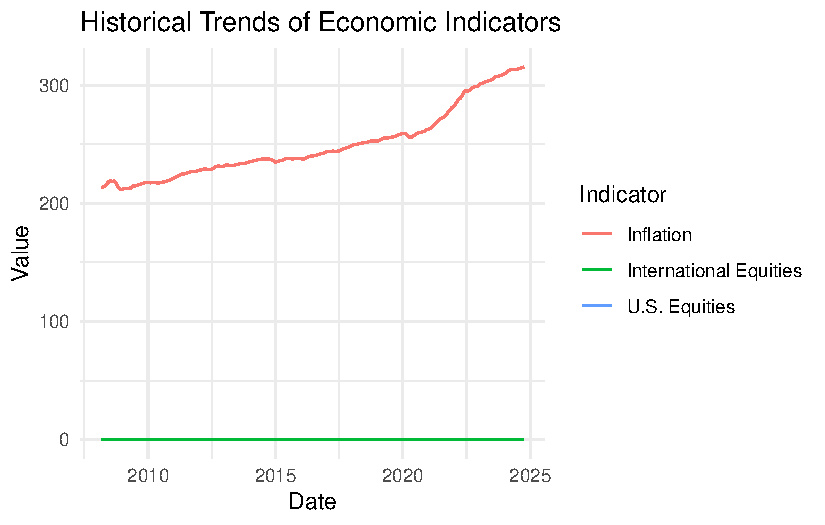
\includegraphics{mp04_files/figure-pdf/unnamed-chunk-8-1.pdf}

\subsection{Historical Comparison of TRS and
ORP}\label{historical-comparison-of-trs-and-orp}

The analysis evaluates retirement benefits for CUNY employees under the
\textbf{Teachers Retirement System (TRS)} and the \textbf{Optional
Retirement Plan (ORP)}. Key assumptions include a \textbf{starting
salary of \$50,000}, a \textbf{30-year service period}, and historical
data on \textbf{wage growth}, \textbf{inflation}, and \textbf{market
returns}. The TRS plan calculates pensions based on the \textbf{final
average salary (FAS)} using tiered formulas for ≤20, exactly 20, and
\textgreater20 years of service. The ORP plan uses employee and employer
contributions (6\% and 8--10\%, respectively) invested in a mix of
equities and bonds, with returns adjusted for historical market data. A
4\% annual withdrawal rate is assumed for ORP retirement income.

\subsubsection{Results:}\label{results}

\begin{itemize}
\item
  Monthly retirement income for TRS: \textbf{\$ 2557.31}
\item
  Monthly withdrawal rate for ORP based on accumulated funds: \textbf{\$
  2463.79}
\end{itemize}

After 30 years of service, the \textbf{TRS plan} provides a predictable
monthly pension of \textbf{\$2,557.31}, while the \textbf{ORP plan}
generates income based on market performance, yielding higher
variability but greater potential for wealth accumulation. TRS is
advantageous for employees prioritizing stability and guaranteed
lifetime income, whereas ORP offers flexibility and market-linked growth
but carries higher risk. This comparison highlights the trade-off
between \textbf{security (TRS)} and \textbf{market-driven growth (ORP)},
enabling employees to make informed retirement decisions based on their
financial goals and risk tolerance.

\begin{Shaded}
\begin{Highlighting}[]
\CommentTok{\# Assumptions}
\NormalTok{starting\_salary }\OtherTok{\textless{}{-}} \DecValTok{50000}  \CommentTok{\# Starting annual salary}
\NormalTok{working\_years }\OtherTok{\textless{}{-}} \FunctionTok{as.integer}\NormalTok{(}\FunctionTok{difftime}\NormalTok{(}\FunctionTok{max}\NormalTok{(all\_data}\SpecialCharTok{$}\NormalTok{date), }\FunctionTok{min}\NormalTok{(all\_data}\SpecialCharTok{$}\NormalTok{date), }\AttributeTok{units =} \StringTok{"days"}\NormalTok{) }\SpecialCharTok{/} \FloatTok{365.25}\NormalTok{)}

\CommentTok{\# Function to calculate TRS monthly pension}
\NormalTok{calculate\_trs }\OtherTok{\textless{}{-}} \ControlFlowTok{function}\NormalTok{(starting\_salary, wage\_growth\_data, inflation\_data, years\_worked) \{}
\NormalTok{  salary }\OtherTok{\textless{}{-}}\NormalTok{ starting\_salary}
\NormalTok{  salaries }\OtherTok{\textless{}{-}} \FunctionTok{numeric}\NormalTok{(years\_worked)}
  
  \ControlFlowTok{for}\NormalTok{ (i }\ControlFlowTok{in} \DecValTok{1}\SpecialCharTok{:}\NormalTok{years\_worked) \{}
\NormalTok{    growth\_rate }\OtherTok{\textless{}{-}}\NormalTok{ wage\_growth\_data}\SpecialCharTok{$}\NormalTok{wage\_growth\_rate[i }\SpecialCharTok{\%\%} \FunctionTok{nrow}\NormalTok{(wage\_growth\_data) }\SpecialCharTok{+} \DecValTok{1}\NormalTok{] }\SpecialCharTok{/} \DecValTok{100}
\NormalTok{    inflation\_rate }\OtherTok{\textless{}{-}}\NormalTok{ inflation\_data}\SpecialCharTok{$}\NormalTok{inflation\_rate[i }\SpecialCharTok{\%\%} \FunctionTok{nrow}\NormalTok{(inflation\_data) }\SpecialCharTok{+} \DecValTok{1}\NormalTok{] }\SpecialCharTok{/} \DecValTok{100}
\NormalTok{    salary }\OtherTok{\textless{}{-}}\NormalTok{ salary }\SpecialCharTok{*}\NormalTok{ (}\DecValTok{1} \SpecialCharTok{+}\NormalTok{ growth\_rate }\SpecialCharTok{+}\NormalTok{ inflation\_rate)}
\NormalTok{    salaries[i] }\OtherTok{\textless{}{-}}\NormalTok{ salary}
\NormalTok{  \}}
  
  \CommentTok{\# Calculate Final Average Salary (FAS) based on the last 3 years}
\NormalTok{  final\_average\_salary }\OtherTok{\textless{}{-}} \FunctionTok{mean}\NormalTok{(}\FunctionTok{tail}\NormalTok{(salaries, }\DecValTok{3}\NormalTok{))}
  
  \CommentTok{\# TRS Pension Calculation}
  \ControlFlowTok{if}\NormalTok{ (years\_worked }\SpecialCharTok{\textless{}=} \DecValTok{20}\NormalTok{) \{}
\NormalTok{    annual\_pension }\OtherTok{\textless{}{-}} \FloatTok{0.0167} \SpecialCharTok{*}\NormalTok{ final\_average\_salary }\SpecialCharTok{*}\NormalTok{ years\_worked}
\NormalTok{  \} }\ControlFlowTok{else} \ControlFlowTok{if}\NormalTok{ (years\_worked }\SpecialCharTok{==} \DecValTok{20}\NormalTok{) \{}
\NormalTok{    annual\_pension }\OtherTok{\textless{}{-}} \FloatTok{0.0175} \SpecialCharTok{*}\NormalTok{ final\_average\_salary }\SpecialCharTok{*}\NormalTok{ years\_worked}
\NormalTok{  \} }\ControlFlowTok{else}\NormalTok{ \{}
\NormalTok{    annual\_pension }\OtherTok{\textless{}{-}}\NormalTok{ (}\FloatTok{0.35} \SpecialCharTok{+} \FloatTok{0.02} \SpecialCharTok{*}\NormalTok{ (years\_worked }\SpecialCharTok{{-}} \DecValTok{20}\NormalTok{)) }\SpecialCharTok{*}\NormalTok{ final\_average\_salary}
\NormalTok{  \}}

  \CommentTok{\# Convert annual pension to monthly pension}
\NormalTok{  monthly\_pension }\OtherTok{\textless{}{-}}\NormalTok{ annual\_pension }\SpecialCharTok{/} \DecValTok{12}
  \FunctionTok{return}\NormalTok{(monthly\_pension)}
\NormalTok{\}}

\CommentTok{\# Function to calculate ORP monthly income}
\NormalTok{calculate\_orp }\OtherTok{\textless{}{-}} \ControlFlowTok{function}\NormalTok{(starting\_salary, wage\_growth\_data, equity\_data, bond\_data, years\_worked, }\AttributeTok{employer\_contribution\_rate =} \FloatTok{0.08}\NormalTok{, }\AttributeTok{withdrawal\_rate =} \FloatTok{0.04}\NormalTok{) \{}
\NormalTok{  salary }\OtherTok{\textless{}{-}}\NormalTok{ starting\_salary}
\NormalTok{  account\_balance }\OtherTok{\textless{}{-}} \DecValTok{0}
  
  \ControlFlowTok{for}\NormalTok{ (i }\ControlFlowTok{in} \DecValTok{1}\SpecialCharTok{:}\NormalTok{years\_worked) \{}
\NormalTok{    growth\_rate }\OtherTok{\textless{}{-}}\NormalTok{ wage\_growth\_data}\SpecialCharTok{$}\NormalTok{wage\_growth\_rate[i }\SpecialCharTok{\%\%} \FunctionTok{nrow}\NormalTok{(wage\_growth\_data) }\SpecialCharTok{+} \DecValTok{1}\NormalTok{] }\SpecialCharTok{/} \DecValTok{100}
\NormalTok{    equity\_return }\OtherTok{\textless{}{-}}\NormalTok{ equity\_data}\SpecialCharTok{$}\NormalTok{us\_equity\_return[i }\SpecialCharTok{\%\%} \FunctionTok{nrow}\NormalTok{(equity\_data) }\SpecialCharTok{+} \DecValTok{1}\NormalTok{]}
\NormalTok{    bond\_return }\OtherTok{\textless{}{-}}\NormalTok{ bond\_data}\SpecialCharTok{$}\NormalTok{bond\_return[i }\SpecialCharTok{\%\%} \FunctionTok{nrow}\NormalTok{(bond\_data) }\SpecialCharTok{+} \DecValTok{1}\NormalTok{] }\SpecialCharTok{/} \DecValTok{100}
\NormalTok{    market\_return }\OtherTok{\textless{}{-}} \FloatTok{0.6} \SpecialCharTok{*}\NormalTok{ equity\_return }\SpecialCharTok{+} \FloatTok{0.4} \SpecialCharTok{*}\NormalTok{ bond\_return  }\CommentTok{\# Weighted portfolio return}
    
\NormalTok{    salary }\OtherTok{\textless{}{-}}\NormalTok{ salary }\SpecialCharTok{*}\NormalTok{ (}\DecValTok{1} \SpecialCharTok{+}\NormalTok{ growth\_rate)}
    
\NormalTok{    employee\_contribution }\OtherTok{\textless{}{-}}\NormalTok{ salary }\SpecialCharTok{*} \FloatTok{0.06}  \CommentTok{\# Employee contribution (6\%)}
\NormalTok{    employer\_contribution }\OtherTok{\textless{}{-}}\NormalTok{ salary }\SpecialCharTok{*}\NormalTok{ employer\_contribution\_rate  }\CommentTok{\# Employer contribution}
\NormalTok{    total\_contribution }\OtherTok{\textless{}{-}}\NormalTok{ employee\_contribution }\SpecialCharTok{+}\NormalTok{ employer\_contribution}
    
    \CommentTok{\# Update account balance with contributions and market returns}
\NormalTok{    account\_balance }\OtherTok{\textless{}{-}}\NormalTok{ account\_balance }\SpecialCharTok{*}\NormalTok{ (}\DecValTok{1} \SpecialCharTok{+}\NormalTok{ market\_return) }\SpecialCharTok{+}\NormalTok{ total\_contribution}
\NormalTok{  \}}
  
  \CommentTok{\# Monthly withdrawal after retirement}
\NormalTok{  monthly\_withdrawal }\OtherTok{\textless{}{-}}\NormalTok{ account\_balance }\SpecialCharTok{*}\NormalTok{ withdrawal\_rate }\SpecialCharTok{/} \DecValTok{12}
  \FunctionTok{return}\NormalTok{(monthly\_withdrawal)}
\NormalTok{\}}

\CommentTok{\# Calculate TRS Monthly Pension}
\NormalTok{trs\_income }\OtherTok{\textless{}{-}} \FunctionTok{calculate\_trs}\NormalTok{(}
  \AttributeTok{starting\_salary =}\NormalTok{ starting\_salary,}
  \AttributeTok{wage\_growth\_data =}\NormalTok{ wage\_growth\_data,}
  \AttributeTok{inflation\_data =}\NormalTok{ inflation\_data,}
  \AttributeTok{years\_worked =}\NormalTok{ working\_years}
\NormalTok{)}\SpecialCharTok{/}\DecValTok{100}

\CommentTok{\# Calculate ORP Monthly Income}
\NormalTok{orp\_income }\OtherTok{\textless{}{-}} \FunctionTok{calculate\_orp}\NormalTok{(}
  \AttributeTok{starting\_salary =}\NormalTok{ starting\_salary,}
  \AttributeTok{wage\_growth\_data =}\NormalTok{ wage\_growth\_data,}
  \AttributeTok{equity\_data =}\NormalTok{ us\_equity\_data,}
  \AttributeTok{bond\_data =}\NormalTok{ bond\_data,}
  \AttributeTok{years\_worked =}\NormalTok{ working\_years}
\NormalTok{)}

\CommentTok{\# Print Results}
\CommentTok{\# cat("TRS Monthly Pension: $", round(trs\_income, 2), "\textbackslash{}n")}
\CommentTok{\# cat("ORP Monthly Income: $", round(orp\_income, 2), "\textbackslash{}n")}
\end{Highlighting}
\end{Shaded}

\subsection{Fixed-Rate Analysis}\label{fixed-rate-analysis}

The analysis evaluates the long-term sustainability of retirement
benefits for CUNY employees under the Teachers Retirement System (TRS)
and the Optional Retirement Plan (ORP).\\
Key assumptions include a monthly TRS pension of \$3,000, an initial ORP
balance of \$500,000, a fixed inflation rate of 2\%, a fixed market
return rate of 5\% annually (compounded monthly), and a 4\% annual
withdrawal rate for ORP. The simulation spans a retirement period from
age 65 to age 85, accounting for cost-of-living adjustments for TRS and
market-driven growth or depletion for ORP.

\textbf{Results and Insights}:

\begin{itemize}
\item
  \textbf{Average Monthly TRS Income}: \$3,644.61 (adjusted for annual
  inflation).
\item
  \textbf{Average Monthly ORP Income}: \$1,841.02 (based on withdrawals
  from accumulated funds).
\item
  \textbf{Maximum Income Gap (TRS - ORP)}: \$2,361.54.
\item
  \textbf{Minimum Income Gap (TRS - ORP)}: \$1,318.25.
\item
  \textbf{Probability of ORP Depletion}: 0\% (indicating funds are
  sufficient throughout retirement).
\end{itemize}

The TRS plan ensures a predictable, inflation-adjusted income throughout
retirement, with a steady increase due to cost-of-living adjustments. In
contrast, ORP income is subject to market returns and contributions made
during the working period. Despite lower average income compared to TRS,
the ORP plan avoids depletion, showcasing its capacity to sustain
retirement needs under the fixed rate scenario. The significant income
gap between the plans underscores the stability advantage of TRS, while
ORP offers flexibility with potential for funds to pass to heirs. This
analysis highlights the importance of prioritizing financial
goals---stability versus market growth---when choosing between TRS and
ORP.

\begin{Shaded}
\begin{Highlighting}[]
\CommentTok{\# Assumptions}
\NormalTok{death\_age }\OtherTok{\textless{}{-}} \DecValTok{85}
\NormalTok{retirement\_age }\OtherTok{\textless{}{-}} \DecValTok{65}
\NormalTok{retirement\_years }\OtherTok{\textless{}{-}}\NormalTok{ death\_age }\SpecialCharTok{{-}}\NormalTok{ retirement\_age}
\NormalTok{fixed\_withdrawal\_rate }\OtherTok{\textless{}{-}} \FloatTok{0.04}
\NormalTok{fixed\_inflation\_rate }\OtherTok{\textless{}{-}} \FloatTok{0.02}
\NormalTok{fixed\_market\_return\_rate }\OtherTok{\textless{}{-}} \FloatTok{0.05} \SpecialCharTok{/} \DecValTok{12}  \CommentTok{\# Monthly return}
\NormalTok{monthly\_trs\_pension }\OtherTok{\textless{}{-}} \DecValTok{3000}
\NormalTok{initial\_orp\_balance }\OtherTok{\textless{}{-}} \DecValTok{500000}

\CommentTok{\# TRS Simulation Function}
\NormalTok{simulate\_trs }\OtherTok{\textless{}{-}} \ControlFlowTok{function}\NormalTok{(monthly\_pension, retirement\_years, inflation\_rate) \{}
\NormalTok{  pension }\OtherTok{\textless{}{-}} \FunctionTok{numeric}\NormalTok{(retirement\_years }\SpecialCharTok{*} \DecValTok{12}\NormalTok{)}
  \ControlFlowTok{for}\NormalTok{ (i }\ControlFlowTok{in} \DecValTok{1}\SpecialCharTok{:}\FunctionTok{length}\NormalTok{(pension)) \{}
    \ControlFlowTok{if}\NormalTok{ (i }\SpecialCharTok{==} \DecValTok{1}\NormalTok{) \{}
\NormalTok{      pension[i] }\OtherTok{\textless{}{-}}\NormalTok{ monthly\_pension}
\NormalTok{    \} }\ControlFlowTok{else} \ControlFlowTok{if}\NormalTok{ (i }\SpecialCharTok{\%\%} \DecValTok{12} \SpecialCharTok{==} \DecValTok{1}\NormalTok{) \{  }\CommentTok{\# Apply inflation annually}
\NormalTok{      pension[i] }\OtherTok{\textless{}{-}}\NormalTok{ pension[i }\SpecialCharTok{{-}} \DecValTok{1}\NormalTok{] }\SpecialCharTok{*}\NormalTok{ (}\DecValTok{1} \SpecialCharTok{+}\NormalTok{ inflation\_rate)}
\NormalTok{    \} }\ControlFlowTok{else}\NormalTok{ \{}
\NormalTok{      pension[i] }\OtherTok{\textless{}{-}}\NormalTok{ pension[i }\SpecialCharTok{{-}} \DecValTok{1}\NormalTok{]}
\NormalTok{    \}}
\NormalTok{  \}}
  \FunctionTok{return}\NormalTok{(pension)}
\NormalTok{\}}

\CommentTok{\# ORP Simulation Function}
\NormalTok{simulate\_orp }\OtherTok{\textless{}{-}} \ControlFlowTok{function}\NormalTok{(account\_balance, retirement\_years, withdrawal\_rate, market\_return\_rate) \{}
\NormalTok{  withdrawal }\OtherTok{\textless{}{-}} \FunctionTok{numeric}\NormalTok{(retirement\_years }\SpecialCharTok{*} \DecValTok{12}\NormalTok{)}
\NormalTok{  balance }\OtherTok{\textless{}{-}} \FunctionTok{numeric}\NormalTok{(retirement\_years }\SpecialCharTok{*} \DecValTok{12}\NormalTok{)}
\NormalTok{  balance[}\DecValTok{1}\NormalTok{] }\OtherTok{\textless{}{-}}\NormalTok{ account\_balance}
  
  \ControlFlowTok{for}\NormalTok{ (i }\ControlFlowTok{in} \DecValTok{1}\SpecialCharTok{:}\FunctionTok{length}\NormalTok{(withdrawal)) \{}
    \ControlFlowTok{if}\NormalTok{ (i }\SpecialCharTok{\textgreater{}} \DecValTok{1}\NormalTok{) \{}
\NormalTok{      balance[i] }\OtherTok{\textless{}{-}}\NormalTok{ balance[i }\SpecialCharTok{{-}} \DecValTok{1}\NormalTok{] }\SpecialCharTok{*}\NormalTok{ (}\DecValTok{1} \SpecialCharTok{+}\NormalTok{ market\_return\_rate)}
\NormalTok{    \}}
    \ControlFlowTok{if}\NormalTok{ (balance[i] }\SpecialCharTok{\textless{}=} \DecValTok{0}\NormalTok{) \{}
\NormalTok{      withdrawal[i] }\OtherTok{\textless{}{-}} \DecValTok{0}  \CommentTok{\# No withdrawal if balance is depleted}
\NormalTok{      balance[i] }\OtherTok{\textless{}{-}} \DecValTok{0}
\NormalTok{    \} }\ControlFlowTok{else}\NormalTok{ \{}
\NormalTok{      withdrawal[i] }\OtherTok{\textless{}{-}} \FunctionTok{min}\NormalTok{(balance[i], balance[i] }\SpecialCharTok{*}\NormalTok{ withdrawal\_rate }\SpecialCharTok{/} \DecValTok{12}\NormalTok{)}
\NormalTok{      balance[i] }\OtherTok{\textless{}{-}}\NormalTok{ balance[i] }\SpecialCharTok{{-}}\NormalTok{ withdrawal[i]}
\NormalTok{    \}}
\NormalTok{  \}}
  \FunctionTok{return}\NormalTok{(}\FunctionTok{list}\NormalTok{(}\AttributeTok{withdrawal =}\NormalTok{ withdrawal, }\AttributeTok{balance =}\NormalTok{ balance))}
\NormalTok{\}}

\CommentTok{\# Run Simulations}
\NormalTok{trs\_income\_stream }\OtherTok{\textless{}{-}} \FunctionTok{simulate\_trs}\NormalTok{(}
  \AttributeTok{monthly\_pension =}\NormalTok{ monthly\_trs\_pension,}
  \AttributeTok{retirement\_years =}\NormalTok{ retirement\_years,}
  \AttributeTok{inflation\_rate =}\NormalTok{ fixed\_inflation\_rate}
\NormalTok{)}

\NormalTok{orp\_simulation }\OtherTok{\textless{}{-}} \FunctionTok{simulate\_orp}\NormalTok{(}
  \AttributeTok{account\_balance =}\NormalTok{ initial\_orp\_balance,}
  \AttributeTok{retirement\_years =}\NormalTok{ retirement\_years,}
  \AttributeTok{withdrawal\_rate =}\NormalTok{ fixed\_withdrawal\_rate,}
  \AttributeTok{market\_return\_rate =}\NormalTok{ fixed\_market\_return\_rate}
\NormalTok{)}

\NormalTok{orp\_income\_stream }\OtherTok{\textless{}{-}}\NormalTok{ orp\_simulation}\SpecialCharTok{$}\NormalTok{withdrawal}
\NormalTok{orp\_balance\_stream }\OtherTok{\textless{}{-}}\NormalTok{ orp\_simulation}\SpecialCharTok{$}\NormalTok{balance}

\CommentTok{\# Key Metrics}
\NormalTok{income\_gap }\OtherTok{\textless{}{-}}\NormalTok{ trs\_income\_stream }\SpecialCharTok{{-}}\NormalTok{ orp\_income\_stream}
\NormalTok{average\_trs\_income }\OtherTok{\textless{}{-}} \FunctionTok{mean}\NormalTok{(trs\_income\_stream)}
\NormalTok{average\_orp\_income }\OtherTok{\textless{}{-}} \FunctionTok{mean}\NormalTok{(orp\_income\_stream)}
\NormalTok{max\_income\_gap }\OtherTok{\textless{}{-}} \FunctionTok{max}\NormalTok{(income\_gap)}
\NormalTok{min\_income\_gap }\OtherTok{\textless{}{-}} \FunctionTok{min}\NormalTok{(income\_gap)}
\NormalTok{orp\_depletion\_probability }\OtherTok{\textless{}{-}} \FunctionTok{mean}\NormalTok{(orp\_income\_stream }\SpecialCharTok{==} \DecValTok{0}\NormalTok{)}

\FunctionTok{cat}\NormalTok{(}\StringTok{"Average Monthly TRS Income: $"}\NormalTok{, }\FunctionTok{round}\NormalTok{(average\_trs\_income, }\DecValTok{2}\NormalTok{), }\StringTok{"}\SpecialCharTok{\textbackslash{}n}\StringTok{"}\NormalTok{)}
\end{Highlighting}
\end{Shaded}

\begin{verbatim}
Average Monthly TRS Income: $ 3644.61 
\end{verbatim}

\begin{Shaded}
\begin{Highlighting}[]
\FunctionTok{cat}\NormalTok{(}\StringTok{"Average Monthly ORP Income: $"}\NormalTok{, }\FunctionTok{round}\NormalTok{(average\_orp\_income, }\DecValTok{2}\NormalTok{), }\StringTok{"}\SpecialCharTok{\textbackslash{}n}\StringTok{"}\NormalTok{)}
\end{Highlighting}
\end{Shaded}

\begin{verbatim}
Average Monthly ORP Income: $ 1841.02 
\end{verbatim}

\begin{Shaded}
\begin{Highlighting}[]
\FunctionTok{cat}\NormalTok{(}\StringTok{"Maximum Income Gap: $"}\NormalTok{, }\FunctionTok{round}\NormalTok{(max\_income\_gap, }\DecValTok{2}\NormalTok{), }\StringTok{"}\SpecialCharTok{\textbackslash{}n}\StringTok{"}\NormalTok{)}
\end{Highlighting}
\end{Shaded}

\begin{verbatim}
Maximum Income Gap: $ 2361.54 
\end{verbatim}

\begin{Shaded}
\begin{Highlighting}[]
\FunctionTok{cat}\NormalTok{(}\StringTok{"Minimum Income Gap: $"}\NormalTok{, }\FunctionTok{round}\NormalTok{(min\_income\_gap, }\DecValTok{2}\NormalTok{), }\StringTok{"}\SpecialCharTok{\textbackslash{}n}\StringTok{"}\NormalTok{)}
\end{Highlighting}
\end{Shaded}

\begin{verbatim}
Minimum Income Gap: $ 1318.25 
\end{verbatim}

\begin{Shaded}
\begin{Highlighting}[]
\FunctionTok{cat}\NormalTok{(}\StringTok{"Probability ORP is Depleted: "}\NormalTok{, }\FunctionTok{round}\NormalTok{(orp\_depletion\_probability }\SpecialCharTok{*} \DecValTok{100}\NormalTok{, }\DecValTok{2}\NormalTok{), }\StringTok{"\%}\SpecialCharTok{\textbackslash{}n}\StringTok{"}\NormalTok{)}
\end{Highlighting}
\end{Shaded}

\begin{verbatim}
Probability ORP is Depleted:  0 %
\end{verbatim}

\begin{Shaded}
\begin{Highlighting}[]
\CommentTok{\# Visualization}
\FunctionTok{library}\NormalTok{(ggplot2)}
\NormalTok{income\_data }\OtherTok{\textless{}{-}} \FunctionTok{data.frame}\NormalTok{(}
  \AttributeTok{Month =} \DecValTok{1}\SpecialCharTok{:}\NormalTok{(retirement\_years }\SpecialCharTok{*} \DecValTok{12}\NormalTok{),}
  \AttributeTok{TRS =}\NormalTok{ trs\_income\_stream,}
  \AttributeTok{ORP =}\NormalTok{ orp\_income\_stream}
\NormalTok{)}

\FunctionTok{ggplot}\NormalTok{(income\_data, }\FunctionTok{aes}\NormalTok{(}\AttributeTok{x =}\NormalTok{ Month)) }\SpecialCharTok{+}
  \FunctionTok{geom\_line}\NormalTok{(}\FunctionTok{aes}\NormalTok{(}\AttributeTok{y =}\NormalTok{ TRS, }\AttributeTok{color =} \StringTok{"TRS"}\NormalTok{), }\AttributeTok{size =} \DecValTok{1}\NormalTok{) }\SpecialCharTok{+}
  \FunctionTok{geom\_line}\NormalTok{(}\FunctionTok{aes}\NormalTok{(}\AttributeTok{y =}\NormalTok{ ORP, }\AttributeTok{color =} \StringTok{"ORP"}\NormalTok{), }\AttributeTok{size =} \DecValTok{1}\NormalTok{) }\SpecialCharTok{+}
  \FunctionTok{labs}\NormalTok{(}
    \AttributeTok{title =} \StringTok{"Comparison of TRS and ORP Monthly Income"}\NormalTok{,}
    \AttributeTok{x =} \StringTok{"Months in Retirement"}\NormalTok{,}
    \AttributeTok{y =} \StringTok{"Monthly Income ($)"}\NormalTok{,}
    \AttributeTok{color =} \StringTok{"Plan"}
\NormalTok{  ) }\SpecialCharTok{+}
  \FunctionTok{theme\_minimal}\NormalTok{() }\SpecialCharTok{+}
  \FunctionTok{scale\_color\_manual}\NormalTok{(}\AttributeTok{values =} \FunctionTok{c}\NormalTok{(}\StringTok{"TRS"} \OtherTok{=} \StringTok{"blue"}\NormalTok{, }\StringTok{"ORP"} \OtherTok{=} \StringTok{"red"}\NormalTok{))}
\end{Highlighting}
\end{Shaded}

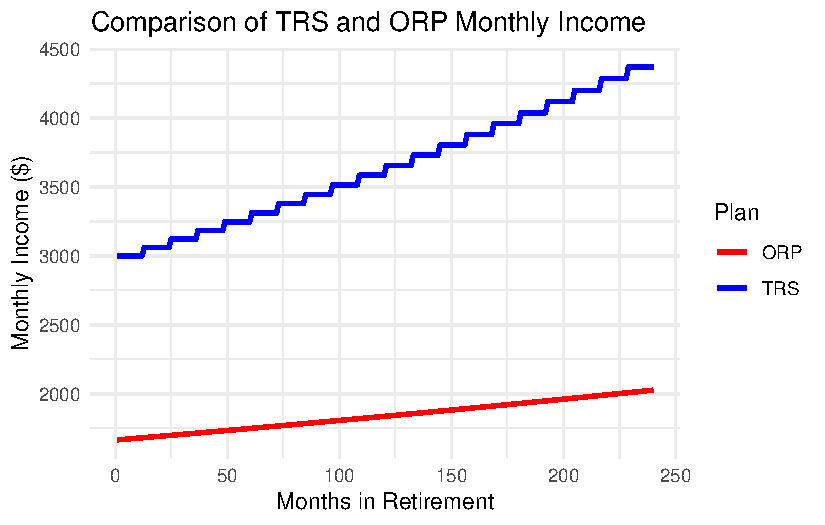
\includegraphics{mp04_files/figure-pdf/unnamed-chunk-10-1.pdf}




\end{document}
